\documentclass[12pt]{article}
\title{Inferring generation-interval distributions from contact tracing data: \\ \emph{in prep, PRSB}}
\author{Sang Woo Park, David Champredon and Jonathan Dushoff}

\usepackage{graphics}
\usepackage{adjustbox}

\newcommand{\eref}[1]{(\ref{eq:#1})}
\newcommand{\fref}[1]{Fig.~\ref{fig:#1}}
\newcommand{\Fref}[1]{Fig.~\ref{fig:#1}}
\newcommand{\sref}[1]{Sec.~\ref{#1}}
\newcommand{\frange}[2]{Fig.~\ref{fig:#1}--\ref{fig:#2}}
\newcommand{\tref}[1]{Table~\ref{tab:#1}}
\newcommand{\tlab}[1]{\label{tab:#1}}

\usepackage{amsthm}
\usepackage{amsmath}
\usepackage{amssymb}
\usepackage{amsfonts}

\usepackage{hyperref}
\usepackage{natbib}
\usepackage{hyperref}
\bibliographystyle{chicago}
\date{\today}

\usepackage{xspace}
\newcommand*{\ie}{i.e.\@\xspace}

\usepackage{color}

\newcommand{\Rx}[1]{\ensuremath{{\mathcal R}_{#1}}} 
\newcommand{\Ro}{\Rx{0}}
\newcommand{\RR}{\ensuremath{{\mathcal R}}}
\newcommand{\Rhat}{\ensuremath{{\hat\RR}}}
\newcommand{\tsub}[2]{#1_{{\textrm{\tiny #2}}}}

\newcommand{\comment}[3]{\textcolor{#1}{\textbf{[#2: }\textsl{#3}\textbf{]}}}
\newcommand{\jd}[1]{\comment{cyan}{JD}{#1}}
\newcommand{\swp}[1]{\comment{magenta}{SWP}{#1}}
\newcommand{\dc}[1]{\comment{blue}{DC}{#1}}
\newcommand{\hotcomment}[1]{\comment{red}{HOT}{#1}}

\begin{document}
\maketitle

\section{Introduction}

%% SWP:
%% Got data from
%% https://www.ncbi.nlm.nih.gov/pubmed/29087987
%% Try and analyze
%% See what's different and understand what they did

An epidemic can be characterized by its speed (exponential growth rate, $r$) and its strength (reproductive number, \RR).
Reproductive number, defined as the average number of secondary cases arising from a primary case, is of particular interest as it provides information about the final size of an epidemic \citep{anderson1991infectious, diekmann1990definition}.
However, directly measuring the reproductive number often requires detailed knowledge of disease natural history and may not be feasible early in an epidemic \swp{Can't figure out what I should cite here; maybe nothing}.
Instead, the reproductive number can be \emph{indirectly} estimated from the exponential growth rate, which can often be estimated from incidence data \citep{mills2004transmissibility, nishiura2009transmission, ma2014estimating}.
These two quantities are linked by generation-interval distributions \citep{wallinga2007generation, park2019practical}.

Generation interval is defined as the time between when a person becomes infected and when that person infects another person.
Due to individual variation in infection time, the observed generation-interval distribution can change depending on when and how it is measured \citep{svensson2007note, kenah2008generation, nishiura2010time, champredon2015intrinsic}.
There are important distinctions to be made when estimating generation intervals: \emph{intrinsic} generation intervals are measured by evaluating the infectiousness of infected people,
%% without regard to actual infection events,
while \emph{observed} generation intervals refer to the time between actual infection events.
Observed generation intervals in turn can be \emph{aggregated} across time, measured \emph{forward} in time by looking at a cohort of individuals infected at the same time and asking when they infected others, or measured \emph{backward in time} by looking at a cohort and asking when their infectors were infected \citep{champredon2015intrinsic}.
% When aggregated generation intervals are observed until a given time in an ongoing epidemic (often via contact tracing), we refer to these as \emph{censored} (or right-censored) intervals.

\jd{Consider rewriting to use early-late as the first-level structure. Early is the part that people focus on most. We could even throw in censorship.}
\swp{Not sure what you mean... I tried to focus on early-late throughout the manuscript}
Early in an epidemic, when depletion of susceptibles is negligible, we expect the forward generation-interval distribution to be similar to the intrinsic generation-interval distribution.
As epidemic progresses, an infector is less likely to infect individuals later in time due to decrease in susceptibles and the distribution of forward generation intervals will be shorter than the intrinsic distribution.
Conversely, when an epidemic is growing exponentially, as often occurs near the beginning of an outbreak, the number of newly infected individuals will be large relative to the number infected earlier on. 
A susceptible individual is thus relatively more likely to be infected by a newly infected individual, and the distribution of backward generation intervals will be shorter than the intrinsic distribution.
When epidemic is subsiding, most infections are caused by the remaining infectors, rather than new infectors, and the backward generation interval will be long \citep{champredon2015intrinsic}.

In practice, generation intervals are often measured by aggregating available information from contact tracing; while an epidemic is ongoing, these measurements are \emph{censored} (or right-censored) at the observation time.
These censored observations can be thought of as a weighted average of backward generation-interval distributions; like them, the observed censored intervals will be shorter than intrinsic distributions early in the epidemic.

Observed generation intervals also vary across space.
In a structured population (that is, any population that does not mix homogeneously), susceptibility will tend to decrease more quickly in the neighborhood of infected individuals than in the general population even in the early phase of an epidemic. 
This means that contacts made late in infection are more likely to be ``masked'' due to infecious contacts that were made earlier.
Therefore, realized generation intervals will be shorter and observed generation intervals may underestimate the intrinsic generation-interval distribution even when population-level susceptibility is very high.
This perspective allows us to reinterpret the finding of \cite{trapman2016inferring} that, given an intrinsic generation interval and an observed growth rate $r$, the reproductive number $\RR$ on various network structures is always smaller on a network than would be predicted from homogeneous mixing.

In this study, we explore the spatiotemporal variation in the observed generation-interval distributions obtained from contact tracing.
We show that directly using the \emph{observed} generation-interval distributions will generally underestimate the reproductive number \RR, while directly using \emph{intrinsic} generation-interval distributions (i.e., estimated from infectiousness profiles) will tend to overestimate \RR.
We discuss statistical approaches to estimating the effective generation-interval distributions and reproductive number of an outbreak from observed generation-interval distributions.
\swp{Come back and fix this}

\swp{I might rename the sections later but I think I like the current order.}
\section{Generation-interval distributions across time}

\subsection{Intrinsic generation-interval distribution}

\begin{figure}[t]
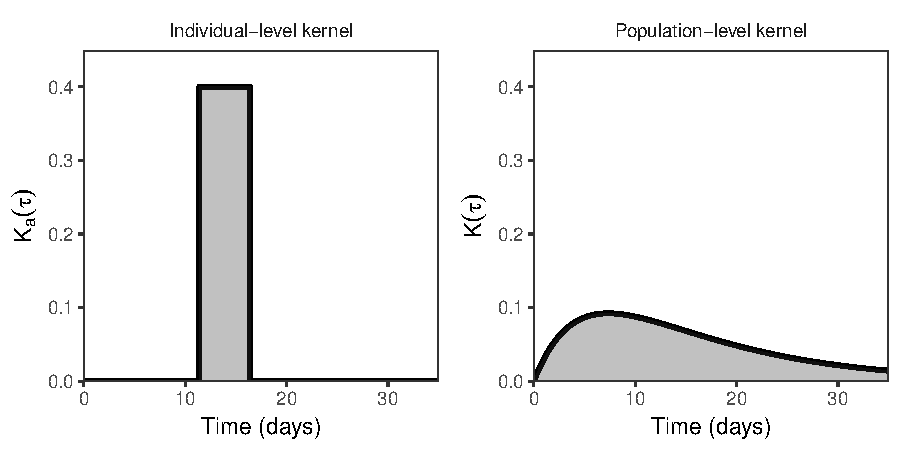
\includegraphics[width=\textwidth]{../fig/individual_and_population.pdf}
\caption{\textbf{Comparison of individual- and population-level kernels.}
(Left) an individual-level kernel of an infected individual with latent period of 11.4 days followed by infectious period of 5 days. 
(Right) a population-level kernel of infected individuals with latent and infectious periods exponentially distributed with means of 11.4 and 5 days, respectively. 
Shaded areas under the curves are equal to individual- and population-level reproductive numbers, both of which are set to 2 in this example.
}
\label{fig:indpop}

\end{figure}

Generation-interval distributions are often viewed from a population-level pespective but we can distinguish population-level distributions from individual-level distributions (\fref{indpop}); 
making this distinction clear will be particularly useful when we discuss spatial components.
An individual-level intrinsic kernel $K_a(\tau)$ describes the rate at which secondary infections are expected to be caused by an infected individual $a$ \citep{svensson2007note, svensson2015influence}.
The population-level kernel is given by integrating over individual variations (e.g., variation in latent and infectious periods):
\begin{equation}
K(\tau) = \int K_a (\tau) dA.
\end{equation}
The population-level kernel describes the rate at which secondary infections are expected to be caused by an \emph{average} infected individual.
\jd{Do we need to worry about assumptions for the rest of this \P? Once we have an aspect space we need to assume that individual properties are independent of risk of infection. Also, since that's wrong on our networks, do we have to figure out why we're approximately saved? I guess because of scaling?}
\swp{What do you mean by individual properties or even scaling?}

There are two components to infection kernels: intrinsic infectiousness of an infected individual (the basic reproductive number) and time distribution of new infections (generation-interval distribution).
The basic reproductive number -- expected number of secondary cases caused by an \emph{average} primary case in a fully susceptible population -- is defined as: 
\begin{equation}
\RR_0 = \int K(t).
\end{equation}
The intrinsic generation-interval distribution is simply the population-level kernel normalized by the basic reproductive number:
\begin{equation}
g(\tau) = \frac{K(t)}{\RR_0}.
\end{equation}

We assume that the disease incidence $i(\tau)$ is the product of the current infectiousness of previously infected individuals and $S(\tau)$, the proportion of the population susceptible.
\begin{equation}
i(\tau) = S(\tau) \int K(s) i(\tau-s) ds = \RR \int g(s) i(\tau-s) ds.
\end{equation}
This model, also referred to as the renewal equation, can represent a wide range of epidemic models \citep{heesterbeek1996concept, diekmann2000mathematical, roberts2004modelling, aldis2005integral, wallinga2007generation, roberts2007model}.
Over a period of time where $S$ remains roughly constant, we would expect approximately exponential growth in $i$; assuming $i(t) = i(0) \exp(r t)$ yields the Euler-Lotka equation \citep{lotka1907relation}, which provides a direct link between speed and strength of an epidemic:
\begin{equation}
\frac{1}{\RR} = \int g(\tau) \exp(-r \tau) d\tau.
\end{equation}

\subsection{Right-censored generation-interval distribution}

\jd{Mathematically, early censored and early backward intervals are the same, but conceptually they're just different. In particular, censoring occurs even with forward tracing.}
\jd{During exponential growth, the theoretical distributions are the same; maybe we should do a tiny bit of that math here so that we can talk more clearly about it.}
\jd{We need to think about exposition. Maybe simple formulae for all of our interval types, both in general and under the assumption of exponential growth.}
\jd{We should be saying that backward $\to$ censored in the limit at the same time we talk about the association below.}
\swp{I tried}

Generation intervals estimated during an outbreak are ``right-censored'', because intervals that end after the observation time are not observed. 
Several studies have associated the backward generation-interval distribution with the observed generation-interval distribution \citep{tomba2010some, nishiura2010time, champredon2015intrinsic, britton2019estimation}, but the backward generation-interval distribution takes into account infections that are only a single generation apart from the focal time.
Instead, contact tracing can be performed over multiple generations, tracing all the way back to the primary case.
The backward generation-interval distribution is mathematically equivalent to the censored generation-interval distribution only during the exponential growth phase, when depletion of the susceptible population is negligible.
However, the exponential growth assumption breaks down rapidly, and it is important to be able to conceptually distinguish the censored generation-interval from the backward generation-interval.
\jd{I hope that none of these papers actually make the mistake that you imply, it's all about the limit.}
\swp{Sure, in the limit they're all same. But we're often not in the limit and contact tracing can be performed beyond the limit. We can make this point.}

The number of infection occuring at time $s$ caused by infectors who were infected at time $s-\tau$ time ago is given by
\begin{equation}
i_{s-\tau}(s) = \RR i(s-\tau) g(\tau) S(s)
\end{equation}
The backward generation-interval distribution, $b_t(\tau)$, describes a distribution of infection that occured $\tau$ time units before the referece time $t$ and is proportional to $i_{t-\tau}(t)$:
\begin{equation}
b_t(\tau) = \frac{i(t-\tau) g(\tau)}{\int_0^t i(t-x) g(x) d\tau}
\end{equation}
On the other hand, the censored generation-interval distribution, $c_t(\tau)$, describes a distribution of \emph{all} infections that are $\tau$ time units apart from any reference time $s$ before $t$ and is proportional to $\int_0^t i_{s-\tau}(s) ds$.
Then, the censored generation-interval distribution is given by
\begin{equation}
c_t(\tau) = \frac{g(\tau) \int_0^t i(s-\tau) S(s) ds}{\int_0^t g(\tau) \int_0^t i(s-\tau) S(s) ds d\tau}
\end{equation}
Alternatively, the censored generatio-interval distribution can be interpreted as a weighted distribution of the backward generation intervals:
\begin{equation}
c_t(\tau) \propto \int_0^t b_s(\tau) S(s) ds.
\end{equation}
Therefore, we expect the backward generation-interval distribution to be equivalent to the censored generation-interval distribution when $S \approx 1$.

\begin{figure}[t]
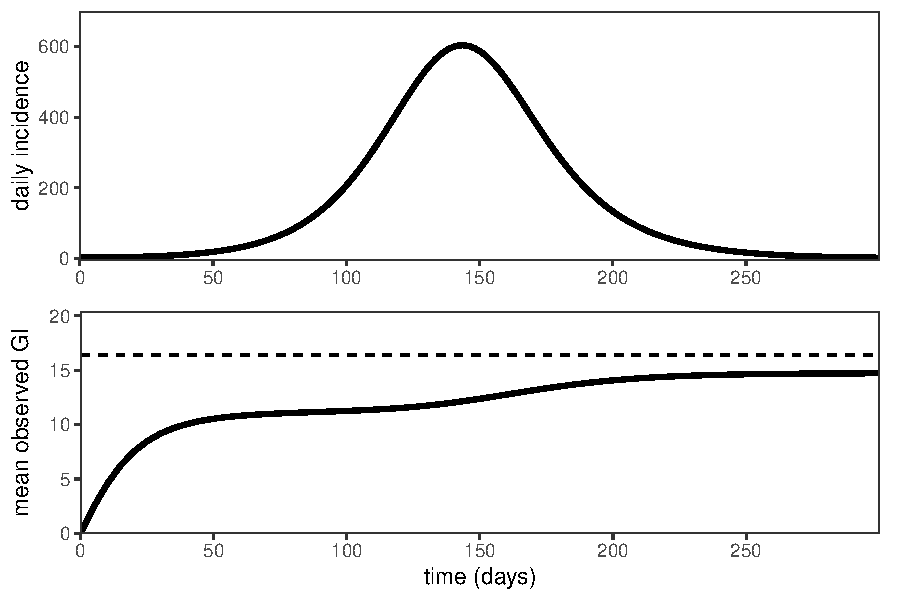
\includegraphics[width=\textwidth]{../fig/temporal_effect.pdf}
\caption{\textbf{Temporal variation in the mean observed generation interval.}
A deterministic Susceptible-Exposed-Infectious-Recovered (SEIR) model was simulated using Ebola-like parameters and the observed (right-censored) mean generation interval was calculated over the course of an epidemic (see methods).
}
\label{fig:censor}
\end{figure}

For a single epidemic, the observed mean generation interval through contact tracing will always be shorter than intrinsic mean generation interval (Figure~\ref{fig:censor}).
There are two reasons for this phenomenon.
First, any infection events that occur after the contact tracing period canonot be observed due to right censoring and short generation intervals are more likely to be observed.
In particular, when an epidemic is growing exponentially ($i(t) = i(0) \exp(rt)$), 
the censored generation-interval distribution is equivalent to the inverse exponentially weighted intrinsic generation-interval distribution \citep{britton2019estimation}:
\begin{equation}
\tsub{c}{exp}(\tau) \propto g(\tau) \exp(-r\tau).
\label{eq:exp}
\end{equation}
% As backward generation-interval distributions are always shorter than the intrinsic generation-interval distribution during the exponential growth period, their weighted average (i.e., the censored intervals) will also be shorter.
Second, decreasing number of susceptibles over the course of an epidemic makes long infections less likely to occur, and the realized intervals will always be shorter \citep{champredon2015intrinsic}.
As a result, even if contact tracing is performed through an entire epidemic, mean generation interval will be underestimated.

When a disease is at (or near) endemic equilibrium, the number of susceptibles remains (approximately) constant over time, and we expect the observed generation-interval distribution to be similar to the intrinsic generation-interval distribution.

\section{Generation-interval distributions across space}

\subsection{Egocentric kernel}

An infected individual may contact the same susceptible individual multiple times, but only the first effective contact gives rise to infection in a given individual (after this, they are no longer susceptible).
Therefore, we expect realized generation intervals to be shorter than intrinsic generation intervals, on average, in a limited contact network.
To explore the effect of multiple contacts on realized generation intervals, we first consider the infection process from an ``egocentric'' point of view, taking into account infectious contacts made by a single infector.
We define the egocentric kernel as the rate at which secondary infections are realized by a single primary case $a$ in the absence of other infectors:
\begin{equation}
\hat{K}_a(\tau) = K_a(\tau) \exp \left(- \delta_a \int_0^\tau K_a(s) ds\right),
\end{equation}
where $K_a(\tau)$ is the individual-level intrinsic kernel and $e^{- \delta_a \int_0^\tau K_a(s) ds}$ is the probability that a susceptible acquaintance has not yet been contacted by individual $a$.
The dilution term, $\delta_a$, models how contacts are distributed among susceptible acquaintances.
For example, when infectious contacts are distributed equally in a homogeneous population, we have $\delta_a = 1/(N-1)$, where $N$ is the population size.

The population-level egocentric kernel is given by integrating over individual variations:
\begin{equation}
\hat{K}(\tau) = \int \hat{K}_a(\tau) dA,
\end{equation}
and the population-level egocentric generation-interval distribution is:
\begin{equation}
\hat{g}(\tau) = \frac{\hat{K}(\tau)}{\int \hat{K} \tau}.
\label{eq:conditional}
\end{equation}
The population-level egocentric generation-interval distribution describes the distribution of times at which secondary infections are realized by an \emph{average} primary case; for brevity we will often omit ``population-level''.

For example, consider a susceptible-exposed-infected-recovered (SEIR) model.
This widely used model assumes that latent and infectious periods are exponentially distributed.
The intrinsic generation-interval distribution that corresponds to this model can be written has \citep{svensson2015influence}:
\begin{equation}
g(\tau) = \frac{\sigma \gamma}{\sigma - \gamma} \left(e^{-\gamma t} - e^{-\sigma t}\right),
\end{equation}
where $1/\sigma$ and $1/\gamma$ are mean latent and infectious periods, respectively.
Assuming that per-pair contact rate is $\lambda$ for any pair, we obtain the following egocentric generation-interval distribution is given by:
\begin{equation}
\hat{g}(\tau) = \frac{\sigma (\gamma + \lambda)}{\sigma - (\gamma + \lambda)} \left(e^{-(\gamma + \lambda)t} - e^{-\sigma t}\right)
\end{equation}
In this scenario, per-pair contact rate effectively decreases mean infectious period: an infected individual can no longer infect anyone (hence no longer infectious) when all its susceptible acquaintances have ben infected.

This calculation can be validated by simulating stochastic infection processes on a ``star'' network (i.e, a single infected individual at the center connected to multiple susceptible individuals who are not connected with each other).
Simulations confirm that in this case the distribution of contact times matches the intrinsic generation-interval distribution, while the distribution of realized generation times matches the egocentric generation-interval distribution (\fref{local}) -- generation times are shorter on average because contacts with already-infected susceptibles do not lead to new infections.

\begin{figure}
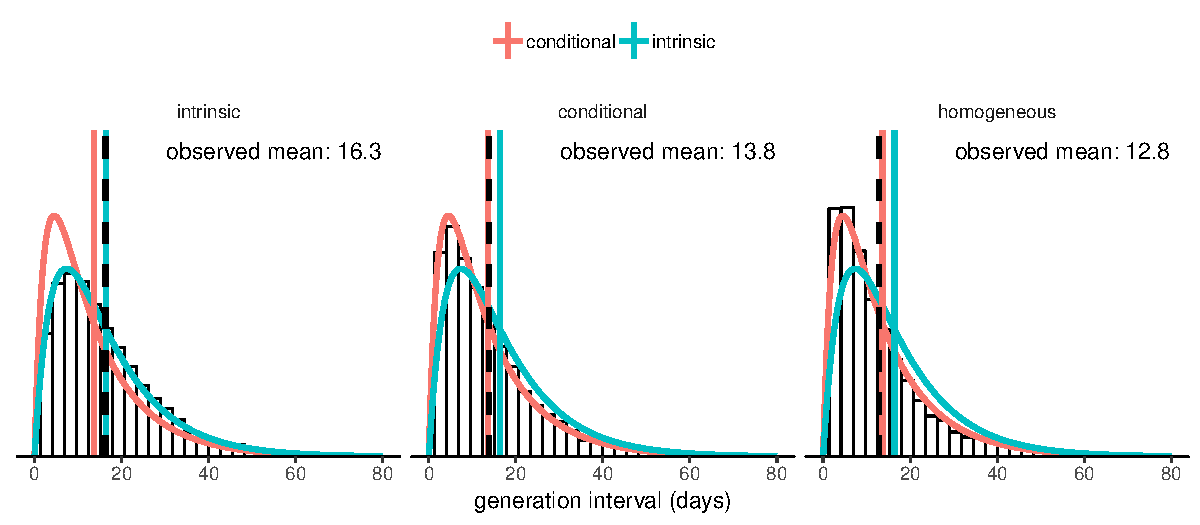
\includegraphics[width=\textwidth]{../fig/local_effect.pdf}
\caption{
\textbf{Spatial effects on realized generation intervals.}
Theoretical distributions and means are shown in color (and are the same in each panel, for reference). Simulated distributions and means are shown in black.
(Left) The intrinsic generation-interval distribution corresponds to all contacts by a focal individual, regardless of whether the individual contacted is susceptible.
(Middle) The egocentric generation-interval distribution corresponds to the distribution of all infectious contacts by the focal individual with susceptible individuals, in the case where the focal individual is the only possible infector (simulated on a star network).
(Right) General spatial distributions are shorter than egocentric distributions, because contacts can be wasted when susceptibles become infected through other routesor (simulated on a homogeneous network).
All graphs were generated using 5000 stochastic simulations were on a network with 5 nodes (1 infector and 4 susceptibles).
}
\label{fig:local}
\end{figure}

The egocentric generation interval \eref{conditional} only explains some of the reduction in generation times that occurs on most networks, however.
Generation intervals are also shortened by indirect connections: a susceptible individual can be infected through another route before the focal individual makes infectious contacts.
Simulations on a small homogeneous network confirm this additional effect (\fref{local}, right panel). 

\jd{I think there's room to be clearer here. All three depletion effects are similar. Should we call them all depletion?: egocentric, local, global?} 
\swp{I like it}
In general, spatial reduction in the mean generation interval can be viewed as an effect of susceptible depletion and can be further classified into three levels: egocentric, local, and global.
Egocentric depletion, as discussed previously, is caused by an infected individual making multiple contacts to the same individual.
Local depletion refers to a depletion of susceptible individuals in a household or neighborhood;
this effect can be observed early in an epidemic, especially in a highly structured population, even if most of the population remains susceptible.
Finally, global depletion refers to overall depeletion of susceptibility as a population-level and explains the underestimation of the mean generation interval, sampled across an entire epidemic (\fref{censor}). 
\jd{I'll have to think about this, or you'll have to explain.} \swp{we changed our local and global explanations so this should be consistent what we said above.}
Although the effect of the overall depletion of susceptible individuals is relatively well-understood \citep{champredon2015intrinsic}, estimating the local effects on observed generation intervals is expected to be a hard problem on realistic networks, although there has been interesting work on spatial cases, particularly on hierarchical networks of households nested within communities (e.g.,  \cite{tomba2010some}). \jd{Don't think we need more than that about Tomba; I wonder if any of Frank Ball's household work could be relevant.}
\jd{The global spatial effect is sort of the non-spatial effect: the overall response to decreasing susceptibles, like in Champredon.}
\swp{Tried to fix this}
\jd{K. I've added at least one new comment in this direction Feb 05 (Tue).}
\swp{Tried to fix this}

\subsection{Linking growth rate and reproductive number}

\swp{I might want to move this paragraph to after equation 13. It doesn't feel like it fits here.}
The intrinsic generation-interval distribution provides a link between the speed (exponential growth rate, $r$) and the strength (reproductive number, $\RR$) of an epidemic via Euler-Lotka equation \citep{lotka1907relation} but assumes a homogeneously mixing population.
Instead, we can derive a relationship between $r$ and $\RR$ that accounts for the egocentric effect using the egocentric generation-interval distribution:
\begin{equation}
\frac{1}{\hat{\RR}} = \int \hat{g}(\tau) \exp(-r \tau) d\tau.
\end{equation}
This is equivalent to the relationship between $r$ and $\RR$ that \cite{trapman2016inferring} derived under a network structure. \swp{Need to confirm; Maybe prove it in appendix or something... will get back to this later}
As the egocentric distribution always has a shorter mean than the intrinsic distribution, \Rhat\ will always be smaller than $\RR$ estimated from the intrinsic distribution.
Similarly, \Rhat\ will be greater than the \emph{true} reproductive number \RR\, since it does not account for depletion of susceptibles by other routes.

\section{Inferring generation-interval distributions from a contact tracing data}

When generation intervals are sampled through contact tracing, there will be four effects present in the sample: (1) right-censoring effect, (2) egocentric effect, (3) local spatial effect and (4) mean susceptible-depletion effect.
We can correct explicitly for the egocentric effect and, in the case of exponential growth, the right-censoring effect.
While the other two effects are difficult to measure, we can make qualitative predictions about their effects on the realized generation intervals and reproductive number. 
\jd{How about: Both local and global depletion\ldots?}
Both local spatial and susceptible depletion effects reduce number of infections that occur and shorten generation intervals but the time scale on which they matter differs:
local spatial effect will be important early in an epidemic whereas the susceptible depletion will be small until sufficient amount of susceptible individuals become infected.
As a result, we expect the initial spread of a disease and the realized reproductive number to be heavily dependent on local spatial and egocentric effects.

Since the right-censoring effect is a sampling artifact, it must be corrected for.
Local and egocentric effects are expected to be embedded within realized generation intervals and do not need to be corrected for as they reflect the unobserved characteristic of a realized epidemic.
We claim that accounting for the right-censoring effect is sufficient and any necessary spatial component will be accounted for implicitly.
Hereafter, we will refer to temporally corrected distribution as the effective generation-interval distribution to contrast from the intrinsic generation-interval distribution; only in a large homogeneously mixing population, the corrected generation-interval distribution will be equivalent to the intrinsic generation-interval distribution.
In this section, we investigate two statistical methods for correcting for temporal bias in a contact tracing data.
Detailed derivations of the two methods can be found in section ???.

We refer to the first method as the population-level method as it relies on the observed distribution aggregated across population.
As the observed generation-interval distribution is a weighted distribution of the effective distribution, the effective distribution can be recovered by taking the inverse of the weights, given by \eref{exp}.
Hence, the population-level method relies on the observed generation intervals and the exponential growth rate \citep{tomba2010some, nishiura2010time}:
\begin{equation}
g(\tau) \propto \tsub{c}{exp}(\tau) \exp(r\tau).
\end{equation}
When the susceptible dynamics is known, this equation can be generalized by using \eref{obsg}.
The population-level method is simple and intuitive, but does not take into account who infected whom; we might therefore expect the individual-level method to be more powerful.

The individual-level method \jd{I don't see how we're assuming this:} assumes that the initial exponential growth phase of an epidemic can be approximated by a Poisson process to derive a likelihood for the observations from each individual:
\begin{equation}
\mathcal{L}(\RR, \theta) = \prod_{j=1}^N \left(\RR^{n_j} \exp \left(- \RR \int_0^{\tsub{t}{censor} - t_j} g(s;\theta) ds \right) \prod_{i=1}^{n_j} g(\tau_{i, j}; \theta) \right),
\end{equation}
where $N$ is the total number of infected individuals, $n_j$ is the number of individuals infected by $j$, $\tsub{t}{censor}$ is the time period which censoring was performed until, $t_j$ is the time at which infector $j$ was infected, $\tau_{i,j}$ is the observed generation interval between infector $j$ and infectee $i$, and $\theta$ is the (vector) parameter of the generation-interval distribution $g$.
\cite{forsberg2008likelihood} proposed a related approach based on discretized incidence reports.

First, we compare how the estimates from the two methods vary across time using a single stochastic simulation on a homogeneous network (\fref{example}).
During the initial exponential growth period (approximately between 9 and 20 weeks), both population-level and individual-level methods yield similar estimates of mean generation interval and reproductive number.
However, we observe opposite trends after the growth period (approximately after 20 weeks). \jd{I kind of feel we're gettting off track here. The main focus should be on early fits, and we should be describing how cool \fref{cmp} is before we wander off into these woods.}
As the population-level method takes a weighted average of the observed distribution, increase in the observed mean generation interval leads to increase in the nonparametric estimates of both mean generation interval and reproductive number.
On the other hand, as the individual-level method assumes a Poisson process with constant proportion of susceptibles, decrease in the number of susceptible is translated to underestimation of both mean generation interval and reproductive number.
we observe gradual increase in the observed mean-generation interval as we aggregate more data, but using the raw observed generation interval distributions always underestimate both mean generation interval and reproductive number, as predicted from the deterministic simulation (Figure~\ref{fig:censor}).
Around the 14th week, reproductive number estimate based on the observed generation interval approximately matches the true reproductive number; this is due to initial overestimation of the initial growth rate and we generally expect reproductive to be underestimated. \swp{Maybe another figure in the supp}

\begin{figure}
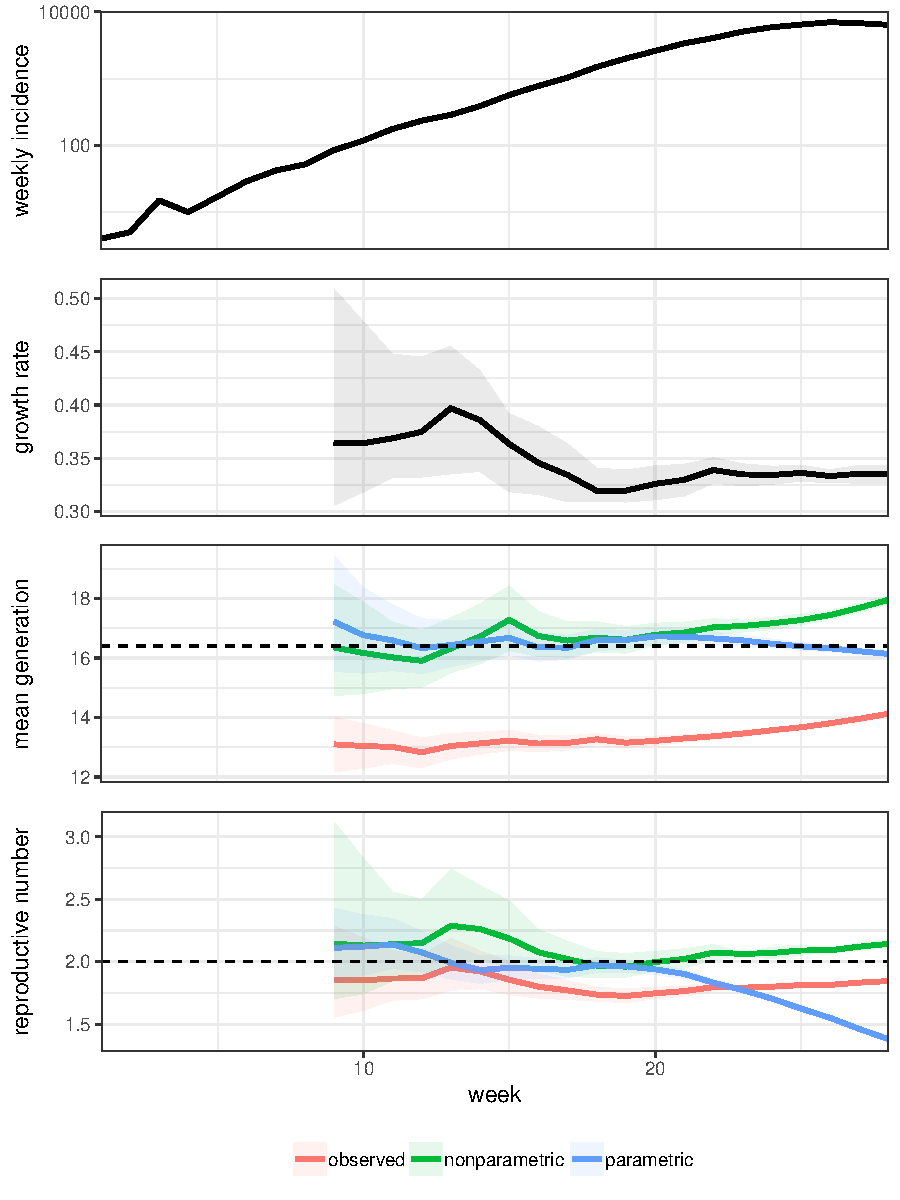
\includegraphics[width=\textwidth]{../fig/example.pdf}
\caption{\swp{Need to re-do this figure; initial overestimation of little $r$ is weird}}
\label{fig:example}
\end{figure}

We compare accuracy and reliability of the two methods during the initial growth period using 100 stochastic simulations on a homogeneous network (Figure~\ref{fig:test}).
We find that the individual-level method provides the most consistent (least variable) estimates.
The population method overestimates reproductive number initially but this is likely to be driven by the initial overestimation of the growth rate as discussed above (Figure~\ref{fig:example}).

\begin{figure}
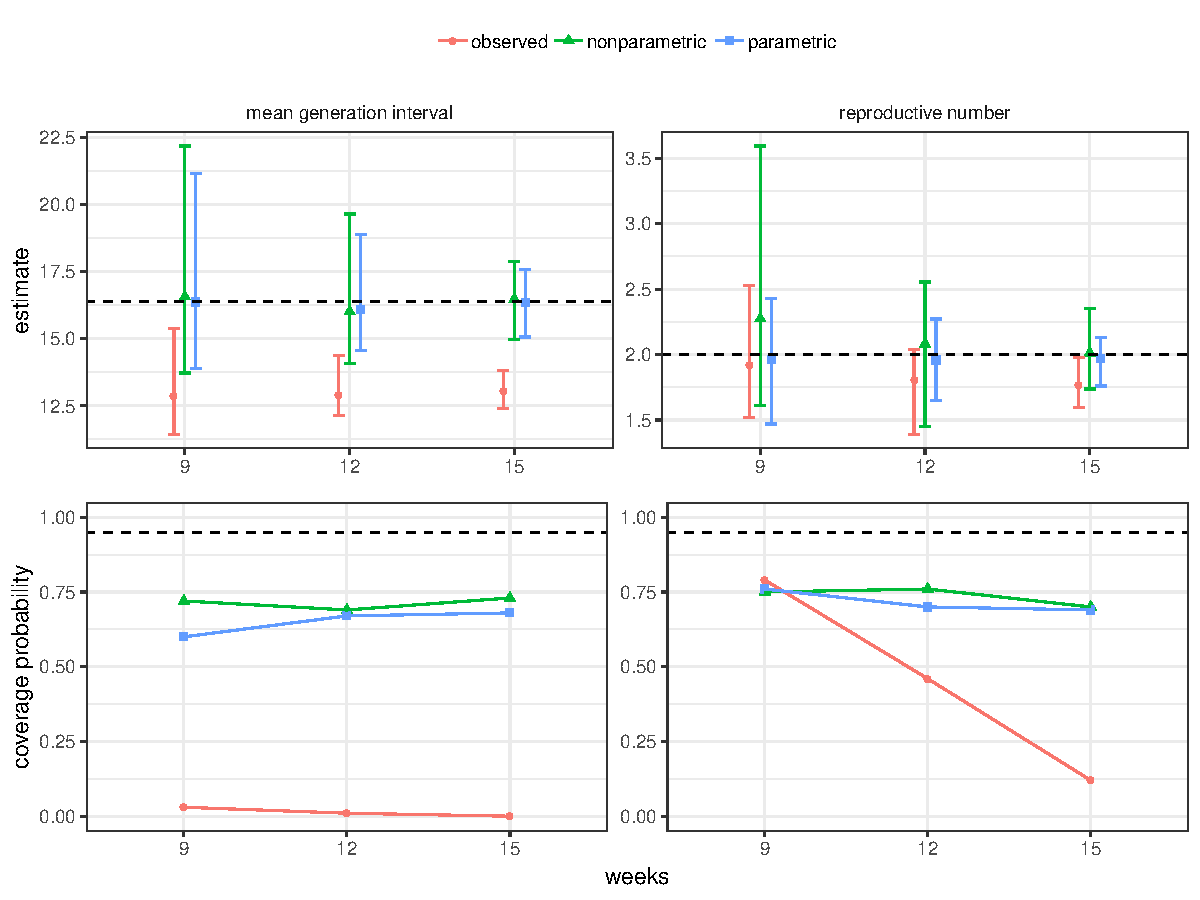
\includegraphics[width=\textwidth]{../fig/compare_methods.pdf}
\caption{\swp{Need to re-do this figure; initial overestimation of little $r$ is weird}.}
\label{fig:test}
\end{figure}

We also compare coverage probabilities of these methods. 
Coverage probabilities are defined as the proportion of confidence intervals that contain the true value in a repeated simulations; for example, a 95\% confidence interval should attain 95\% coverage probability by its definition.
Surprisingly, both methods only attain approximately 70\% coverage.
Even though the gamma distribution looks indistinguishable from the shape of the intrinsic generation-interval distribution, making a wrong distributional assumption leads to narrow confidence intervals.
To confirm that the undercoverage is caused by distribuional assumption, we simulated an epidemic using gamma intrinsic generation-interval and found that fitting the true shape yields nominal coverage (see Appendix).
These results are particularly alarming because shape of the generation-interval distribution have often been assumed in outbreak analyses and it is impossible to know the true shape of the distribution [CITE].

\begin{figure}
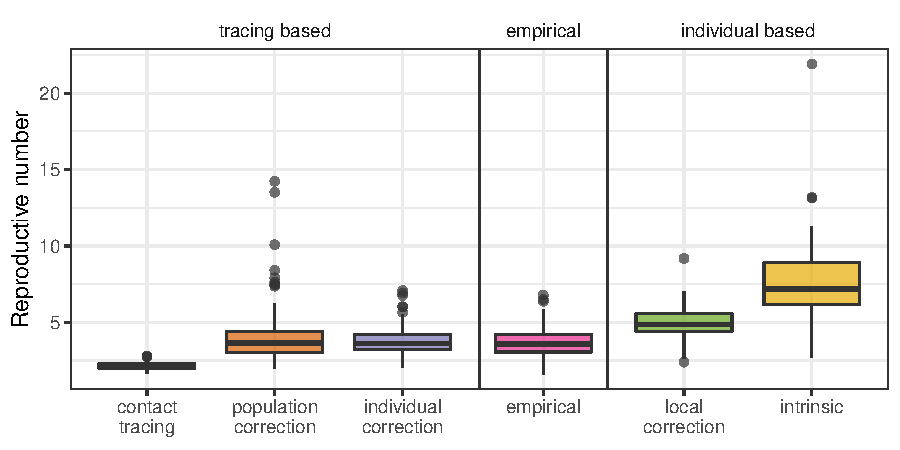
\includegraphics[width=\textwidth]{../fig/cmp_reproductive.pdf}
\caption{\textbf{Comparison of estimates of reproductive number based on various methods}
Using the observed generation-interval distributions without correcting for right-censoring severely underestimates the reproductive number.
Similarly, using intrinsic and egocentric generation-interval distributions without accounting for local spatial effects overestimates the reproductive number.
Both population-level and individual-level methods provide estimates of reproductive number that are consistent with the empirical estimates, which we define as the average number of secondary cases generated by the first 100 infected individuals.
100 stochastic simulations were performed on an empirical network [CITE] using Ebola-like parameters (latent period = 11.4 days and infectious period = 5 days).
}
\label{fig:cmp}
\end{figure}

%% TODO: put SEIR in main text and show SE2IR in appendix for consistency
Finally, we simulate 100 epidemics with Ebola-liked parameters on an empirical network [CITE] and compare the estimates of reproductive number based on different methods with empirical reproductive numbers, which we define as the average number of secondary cases generated by the first 100 infected individuals (\fref{cmp}).
As we predicted earlier, calculating reproductive number based on the intrinsic generation-interval distribution overestimates the empirical reproductive number;
estimates based on the egocentric generation-interval distribution (\eref{conditional}) are closer to empirical reproductive numbers but still suffer from overestimation as they do not account for indirect spatial effects.
Direct estimates based on contact tracing data severely underestimates the empirical estimates.
Both population and individual corrections provide similar estimates to empirical reproductive numbers.
For smaller values of \RR, we expect the differences to become smaller. 

\clearpage

\section{Discussion}

\section{Methods}

The first method is a non-parametric method.
Recall that the observed generation-interval distribution is a weighted intrinsic generation-interval distribution (equation~\ref{eq:obsg}). 
Then, the intrinsic generation-interval distribution can be obtained by taking the inverse weight:
\begin{equation}
g(\tau) \propto c_t(\tau) \frac{1}{\int_{0}^t i(s-\tau) S(s) ds}
\end{equation}
However, this method requires a knowledge of susceptible dynamics and may difficult to use in practice.
Instead, during the exponential period, the generation-interval distribution is
\begin{equation}
g(\tau) \propto \tsub{c}{exp}(\tau) \exp(r\tau)
\end{equation}
and the reproductive number is
\begin{equation}
\RR = \int \tsub{c}{exp}(\tau) \exp(r\tau) d\tau.
\end{equation}
Note that applying the Lotka-Euler equation directly to the observed generation intervals will always underestimate the reproductive number:
\begin{equation}
\int_0^\infty \tsub{g}{exp}(\tau) \exp(r\tau) d\tau > \left(\int_0^\infty \tsub{g}{exp}(\tau). \exp(-r\tau) d\tau\right)^{-1}
\end{equation}

Finally, we obtain an estimator for mean generation interval and the reproductive number:
\begin{equation}
\begin{aligned}
\hat{G} &= \frac{\sum_{i} \exp(r c_i) c_i}{\sum_{i} \exp(r c_i)},\\
\hat{\RR} &= \sum_{i} \exp(r c_i),
\end{aligned}
\end{equation}
where $r$ is the exponential growth rate and $c_i$ is an individual generation interval sample.

\section{Appendix}

These are notes for now ... Need to move them elsewhere and change notation... but this is part of our figure for empirical network ...

$$
1 = \kappa \phi_L(\alpha) \frac{\lambda^{(net)}}{\alpha + \lambda^{(net)}} (1 - \phi_I(\alpha+\lambda^{(net)}))
$$
where in our specific example,
$$
\phi_L(\alpha) = \frac{4 \delta^2}{(2 \delta + \alpha)^2}
$$
and so we have
$$
1 = \frac{4 \delta^2}{(2 \delta + \alpha)^2} \frac{\kappa \lambda^{(net)}}{\lambda^{(net)} + \alpha + \gamma},
$$
which suggests that
$$
\lambda^{(net)} = \frac{(2\delta + \alpha)^2 (\alpha + \gamma)}{(\kappa - 1) 4 \delta^2 - 4 \delta \alpha - \alpha^2}
$$
We can substitute into the following equation to obtain the $r$ and $\RR$ relationship:
$$
\RR = \kappa \frac{\lambda^{(net)}}{\lambda^{(net)} + \gamma}
$$

\bibliography{network}
\end{document}
